\hypertarget{wspr-encoder}{%
\section{WSPR encoder}\label{wspr-encoder}}

This is an educational WSPR encoder python program. Notes are by Philip
Leong (VK2APL) for ELEC3607 at the University of Sydney. *
\url{https://wsjt.sourceforge.io/refs.html} * WSPR implementation notes
on which this is based \url{http://g4jnt.com/WSPR_Coding_Process.pdf} *
\url{https://www.zaarc.org/WSPR_2.0_User.pdf}

\begin{lstlisting}[language=Python]
#!/usr/bin/env python3
"""
wspr_encoder.py -- Generate a WSPR transmission as a 12000 Hz WAV file.

WSPR (Weak Signal Propagation Reporter) encodes a callsign, 4-character
Maidenhead grid locator and transmit power into 162 4-FSK symbols transmitted
over ~110.6 seconds.  The four tones are spaced 12000/8192 ≈ 1.4648 Hz apart.
"""

import sys
import argparse
import wave
import math
import numpy as np

# ---------------------------------------------------------------------------
# WSPR protocol constants
# ---------------------------------------------------------------------------
WSPR_SAMPLE_RATE = 12000          # standard processing rate
WSPR_SYM_SAMP    = 8192           # samples per symbol at 12000 Hz
WSPR_SYMBOLS     = 162            # total symbols per transmission
WSPR_TONE_SEP    = WSPR_SAMPLE_RATE / WSPR_SYM_SAMP   # ≈ 1.4648 Hz
WSPR_DURATION    = WSPR_SYMBOLS * WSPR_SYM_SAMP / WSPR_SAMPLE_RATE  # ≈ 110.6 s
\end{lstlisting}

\hypertarget{encode-a-wspr-message-and-return-wspr_symbols-symbols-each-0-3.}{%
\subsection{Encode a WSPR message and return WSPR\_SYMBOLS symbols (each
0-3).}\label{encode-a-wspr-message-and-return-wspr_symbols-symbols-each-0-3.}}

\hypertarget{standard-message-format}{%
\subsubsection{Standard Message Format}\label{standard-message-format}}

The standard message is callsign + 4 digit locator + dBm transmit power.

Input data * Callsign with a maximum of six characters consisting only
of A-Z, 0-9 and {[}space{]} * Four digit locator (such as IO90) * Power
level representing dBm from 0 to 60. All letters are converted upper
case

Standard message: callsign + 4-digit locator + dBm K1ABC FN20 37 *
Standard message components after lossless compression: 28 bits for
callsign, 15 for locator, 7 for power level, 50 bits total.

The additional message types below are not supported by this notebook: *
Messages with a compound callsign and/or 6-digit locator use a two-
transmission sequence. The first transmission carries compound callsign
and power level, or standard callsign, 4-digit locator, and power level;
the second transmission carries a hashed callsign, 6-digit locator, and
power level. Examples: PJ4/K1ABC 37 K1ABC FN42 37 FK52UD 37 FN42AX 37
Add-on prefixes can be up to three alphanumeric characters; add-on
suffixes can be a single letter or one or two digits.

\begin{lstlisting}[language=Python]
callsign="VK2ABC"
locator="QF56"
power=3
freq=1500
pad=2
rate=WSPR_SAMPLE_RATE
out="wspr_{}_{}_{}.wav".format(callsign, locator, power)
\end{lstlisting}

\begin{lstlisting}[language=Python]
_CHARS = '0123456789ABCDEFGHIJKLMNOPQRSTUVWXYZ '

# This is the _CHARS lookup and indexes
for i in _CHARS:
    print((i, _CHARS.index(i)), end='')
\end{lstlisting}

\begin{lstlisting}
('0', 0)('1', 1)('2', 2)('3', 3)('4', 4)('5', 5)('6', 6)('7', 7)('8', 8)('9', 9)('A', 10)('B', 11)('C', 12)('D', 13)('E', 14)('F', 15)('G', 16)('H', 17)('I', 18)('J', 19)('K', 20)('L', 21)('M', 22)('N', 23)('O', 24)('P', 25)('Q', 26)('R', 27)('S', 28)('T', 29)('U', 30)('V', 31)('W', 32)('X', 33)('Y', 34)('Z', 35)(' ', 36)
\end{lstlisting}

\hypertarget{callsign}{%
\subsection{Callsign}\label{callsign}}

The third character MUST be a number. To cope with callsigns that start
letter followed by a number, a space is appended to the front if
necessary. So, for example, G4JNT will become {[}sp{]}G4JNT whereas
GD4JNT stays as-is.

Short callsigns are then further padded out to six characters by
appending spaces to the end.

The 37 allowed characters are allocated values from 0 to 36 such that
`0' -- `9' give 0 -- 9, `A' to `Z' give 10 to 35 and {[}space{]} is
given the value 36.

Further coding rules on callsigns mean that the final three characters
(of the now padded out callsign) can only be letters or {[}sp{]} so will
only take the values 10 -- 36.

With the characters, designated {[}Ch X{]}, taking on values from 0 to
36 as defined, the callsign is now compressed into a single integer N by
successively building up.

\begin{lstlisting}
N1 = [Ch 1] The first character can take on any of the 37 values including [sp],
N2 = N1 * 36 + [Ch 2] but the second character cannot then be a space so can have 36 values
N3 = N2 * 10 + [Ch 3] The third character must always be a number, so only 10 values are possible.
N4 = 27 * N3 + [Ch 4] – 10]
N5 = 27 * N4 + [Ch 5] – 10] Characters at the end cannot be numbers,
N6 = 27 * N5 + [Ch 6] – 10] so only 27 values are possible.
(In practice N will just be one 32 bit integer variable that can be built up in stages)
\end{lstlisting}

Giving an absolute maximum value for N of:

37 * 36 * 10 * 27 * 27 * 27 = 262177560

Which is just comfortably less than 228 = 268435456 and means the
callsign can be represented by 28 bits with a range of codes left over
for the future, eg. For allocation to special cases and flags.

\begin{lstlisting}[language=Python]
# ---------------------------------------------------------------------------
# Source encoder
# ---------------------------------------------------------------------------
def _encode_callsign(call: str) -> int:
    """Pack a callsign into a 28-bit integer."""
    call = call.upper().strip()
    # 1-letter prefix (G4JNT → ' G4JNT'): 2nd char is digit, prepend space
    # 2-letter prefix (VK2XX, K1ABC): pad right with spaces
    if len(call) >= 2 and call[1].isdigit():
        call = (' ' + call).ljust(6)[:6]
    else:
        call = call.ljust(6)[:6]
    print("Encoding", call)
    n = _CHARS.index(call[0])
    print("n={} (call[0]={}, index={})".format( n, call[0], _CHARS.index(call[0])))
    n = n * 36 + _CHARS.index(call[1])
    print("n=n*36+{}={} (call[1]={}, index={})".format(_CHARS.index(call[1]), n, call[1], _CHARS.index(call[1])))
    n = n * 10 + _CHARS.index(call[2])
    print("n=n*10+{}={} (call[2]={}, index={})".format(_CHARS.index(call[2]), n, call[2], _CHARS.index(call[2])))
    n = n * 27 + (_CHARS.index(call[3]) - 10)
    print("n=n*27+{}-10={} (call[2]={}, index={})".format(_CHARS.index(call[3]), n, call[3], _CHARS.index(call[3])))
    n = n * 27 + (_CHARS.index(call[4]) - 10)
    print("n=n*27+{}-10={} (call[2]={}, index={})".format(_CHARS.index(call[4]), n, call[4], _CHARS.index(call[4])))
    n = n * 27 + (_CHARS.index(call[5]) - 10)
    print("n=n*27+{}-10={} (call[2]={}, index={})".format(_CHARS.index(call[5]), n, call[5], _CHARS.index(call[5])))
    return n
    
n      = _encode_callsign(callsign)
\end{lstlisting}

\begin{lstlisting}
Encoding VK2ABC
n=31 (call[0]=V, index=31)
n=n*36+20=1136 (call[1]=K, index=20)
n=n*10+2=11362 (call[2]=2, index=2)
n=n*27+10-10=306774 (call[2]=A, index=10)
n=n*27+11-10=8282899 (call[2]=B, index=11)
n=n*27+12-10=223638275 (call[2]=C, index=12)
\end{lstlisting}

\hypertarget{locator}{%
\subsection{Locator}\label{locator}}

Designating the four locator characters as {[}Loc 1{]} to {[}Loc 4{]},
the first two can each take on the 18 values A to R only so are
allocated numbers from 0 -- 17. The second pair can take only the values
0 -- 9.

Another integer M1 is formed from:

\begin{lstlisting}
M1 = (179 - 10 * [Loc 1] - [Loc 3] ) * 180 + 10 * [Loc 2] + [Loc 4]
\end{lstlisting}

Which gives a range of values from AA00 (32220) to RR99 (179), which
comfortably fit into a 15 bit representation (215 = 32768), leaving
spare codes for further enhancements. Power Level

Power level, {[}Pwr{]} is taken as a value from 0 -- 60. Although only
certain values will work with the WSJT / WSPR software (just those
ending in 0, 3 or 7) any of the possible 61 values will be encoded;
Illegal values are labelled when decoded.

Power is encoded into M by :

\begin{lstlisting}
M = M1 * 128 + [Pwr] + 64
\end{lstlisting}

Which gives a final range of values for M up to a maximum of 4124287,
and fits into 22 bits (222 = 4194304)

\begin{figure}
\centering
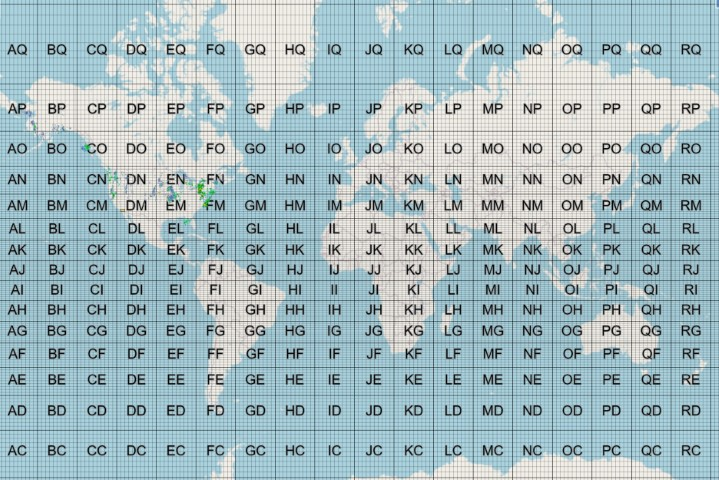
\includegraphics{maidenhead.jpg}
\caption{image.jpg}
\end{figure}

\begin{lstlisting}[language=Python]
def _encode_locator_power(loc: str, pwr: int) -> int:
    """Pack a 4-char Maidenhead locator and power (dBm) into a 22-bit integer."""
    loc = loc.upper()
    print("Encoding loc=", loc)
    m  = (179 - 10 * (_CHARS.index(loc[0]) - _CHARS.index('A')) - int(loc[2])) * 180
    print("m=197-10*({}-{})-{}*100={} (ord(loc[0])={}, int(loc[2]))={}".format(ord(loc[0]), ord('A'), int(loc[2]), m, ord(loc[0]), int(loc[2])))
    m += 10 * (_CHARS.index(loc[1]) - _CHARS.index('A')) + int(loc[3])
    print("m+= 10*({}-{}) + {}={} (_CHARS.index(loc[1])={}, int(loc[3])={})".format(_CHARS.index(loc[1]), _CHARS.index('A'), int(loc[3]), m, ord(loc[1]), int(loc[3])))  
    m = m * 128 + pwr + 64
    print("m = m * 128 + {} + 64={} (pwr={})".format(pwr, m, pwr))
    return m

m      = _encode_locator_power(locator, power)
\end{lstlisting}

\begin{lstlisting}
Encoding loc= QF56
m=197-10*(81-65)-5*100=2520 (ord(loc[0])=81, int(loc[2]))=5
m+= 10*(15-10) + 6=2576 (_CHARS.index(loc[1])=70, int(loc[3])=6)
m = m * 128 + 3 + 64=329795 (pwr=3)
\end{lstlisting}

\hypertarget{bit-packing}{%
\subsection{Bit Packing}\label{bit-packing}}

The total source data has now been reduced to 50 bits of data: 28 for
the callsign in N, and 15 for the locator and 7 for the power in M. A
few special cases of coding are available for future enhancements like
text messages, but these are not be covered here.

The two integers N and M are truncated and combined so the 50 bits sit
end-to-end as callsign-locator-power. These are placed into an array of
eleven 8-bit bytes c{[}0{]} to c{[}10{]}, so the first element c{[}0{]}
contains the most significant 8 bits part of the callsign, c{[}1{]} the
next 8 bits and so on.

Note that c{[}3{]} contains both the 4 LSBs of the callsign and 4 MSBs
of the locator, and that c{[}6{]} contains just the two LSBs of M
occupying the most significant bit positions.

The lowest six bits of c{[}6{]} are set to 0, with the remaining
bytearray elements {[}c7{]} to c{[}10{]} set to zero. Only the left-most
81 of these 88 total bits are subsequently used.

An alternative view is to imagine them as an 81 character-long string
containing characters 0 and 1 only.

\begin{lstlisting}[language=Python]
def _pack_50_bits(n: int, m: int) -> list:
    """Combine 28-bit N and 22-bit M into an 81-bit list (50 data + 31 zeros)."""
    combined = (n << 22) | m
    print("Combined=({} << 22) | {} = {} ({:032b})".format(n, m, combined, combined))
    return [(combined >> i) & 1 for i in range(49, -1, -1)] + [0] * 31

bits   = _pack_50_bits(n, m)
\end{lstlisting}

\begin{lstlisting}
Combined=(223638275 << 22) | 329795 = 938006911715395 (11010101010001110011000000110001010000100001000011)
\end{lstlisting}

\hypertarget{convolutional-encoding-forward-error-correction}{%
\subsection{Convolutional Encoding / Forward Error
Correction}\label{convolutional-encoding-forward-error-correction}}

The data is now expanded to add Forward Error Correction (FEC) with a
rate ½, constraint length 32, convolutional encoder. The 81 bits
(including the 31 trailing zeros) are read out MSB first in the order:

\begin{lstlisting}
c[0] MSB ... c[0] LSB., c[1] MSB ... c[1] LSB ... etc ... c[11]
\end{lstlisting}

(or adopting the alternative view, one-at-a-time from the left hand end
of the string)

The bits are clocked simultaneously into the right hand side, or least
significant position, of two 32 bit shift registers {[}Reg 0{]} and
{[}Reg 1{]}. Each shift register feeds an ExclusiveOR parity generator
from feedback taps described respectively by the 32 bit values
0xF2D05351 and 0xE4613C47.

Parity generation starts immediately the first bit appears in the
registers (which must be initially cleared) and continues until the
registers are flushed by the final 31st zero being clocked into them.

Each of the 81 bits shifted in generates a parity bit from each of the
generators , a total of 162 bits in all. For each bit shifted in, the
resulting two parity bits are taken in turn, in the order the two
feedback tap positions values are given, to give a stream of 162 output
bits.

\hypertarget{parity-generation-process-summary}{%
\subsection{Parity Generation Process
Summary}\label{parity-generation-process-summary}}

The expansion from 50 source data bits to 162 has added sufficient
redundancy in an optimised manner to give a code capable of very strong
Forward Error Correction against random errors.

\begin{itemize}
\tightlist
\item
  Shift the next source bit into the LSB of {[}Reg 0{]} and {[}Reg 1{]}
  (existing bits shift left)
\item
  Take the contents of {[}Reg 0{]}
\item
  AND with 0xF2D05351
\item
  Calculate the single bit parity (XOR) of the resulting sum
\item
  Append to the output data stream
\item
  Take the contents of {[}Reg 1{]}
\item
  AND with 0xE4613C47
\item
  Calculate the single bit parity (XOR) of the resulting sum
\item
  Append to the output data stream
\end{itemize}

F2D05351 → 1111 0010 1101 0000 0101 0011 0101 0001

\begin{figure}
\centering
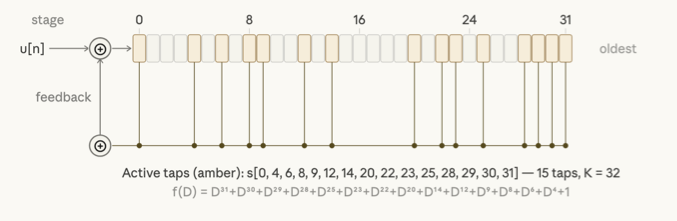
\includegraphics{feedforward_encoder_F2D05351.png}
\caption{image.png}
\end{figure}

\begin{lstlisting}[language=Python]
# Convolutional encoder polynomials  (rate-1/2, constraint length K=32)
POLY1 = 0xF2D05351
POLY2 = 0xE4613C47

# ---------------------------------------------------------------------------
# Convolutional encoder  (rate-1/2, K=32)
# ---------------------------------------------------------------------------
def _parity(x: int) -> int:
    x ^= x >> 16; x ^= x >> 8; x ^= x >> 4; x ^= x >> 2; x ^= x >> 1
    return x & 1


def _conv_encode(bits: list) -> list:
    """Encode 81 source bits → 162 coded bits."""
    reg = 0
    i = 0
    out = []
    print("bits=", ''.join(str(item) for item in bits))
    for b in bits:
        reg = ((reg << 1) | b) & 0xFFFFFFFF
        print("reg[{:02}]={:032b}".format(i, reg), end='')
        print(" (p1,p2)=({},{}) -> ({},{})".format(hex(reg & POLY1), hex(reg & POLY2), _parity(reg & POLY1), _parity(reg & POLY2)))
        out.append(_parity(reg & POLY1))
        out.append(_parity(reg & POLY2))
        i = i + 1
    return out

coded  = _conv_encode(bits)
\end{lstlisting}

\begin{lstlisting}
bits= 110101010100011100110000001100010100001000010000110000000000000000000000000000000
reg[00]=00000000000000000000000000000001 (p1,p2)=(0x1,0x1) -> (1,1)
reg[01]=00000000000000000000000000000011 (p1,p2)=(0x1,0x3) -> (1,0)
reg[02]=00000000000000000000000000000110 (p1,p2)=(0x0,0x6) -> (0,0)
reg[03]=00000000000000000000000000001101 (p1,p2)=(0x1,0x5) -> (1,0)
reg[04]=00000000000000000000000000011010 (p1,p2)=(0x10,0x2) -> (1,1)
reg[05]=00000000000000000000000000110101 (p1,p2)=(0x11,0x5) -> (0,0)
reg[06]=00000000000000000000000001101010 (p1,p2)=(0x40,0x42) -> (1,0)
reg[07]=00000000000000000000000011010101 (p1,p2)=(0x51,0x45) -> (1,1)
reg[08]=00000000000000000000000110101010 (p1,p2)=(0x100,0x2) -> (1,1)
reg[09]=00000000000000000000001101010101 (p1,p2)=(0x351,0x45) -> (1,1)
reg[10]=00000000000000000000011010101010 (p1,p2)=(0x200,0x402) -> (1,0)
reg[11]=00000000000000000000110101010100 (p1,p2)=(0x150,0xc44) -> (1,0)
reg[12]=00000000000000000001101010101000 (p1,p2)=(0x1200,0x1800) -> (0,0)
reg[13]=00000000000000000011010101010001 (p1,p2)=(0x1151,0x3441) -> (1,1)
reg[14]=00000000000000000110101010100011 (p1,p2)=(0x4201,0x2803) -> (1,0)
reg[15]=00000000000000001101010101000111 (p1,p2)=(0x5141,0x1447) -> (1,0)
reg[16]=00000000000000011010101010001110 (p1,p2)=(0x200,0x12806) -> (1,1)
reg[17]=00000000000000110101010100011100 (p1,p2)=(0x5110,0x11404) -> (0,0)
reg[18]=00000000000001101010101000111001 (p1,p2)=(0x211,0x2801) -> (1,1)
reg[19]=00000000000011010101010001110011 (p1,p2)=(0x5051,0x11443) -> (1,0)
reg[20]=00000000000110101010100011100110 (p1,p2)=(0x100040,0x2846) -> (0,1)
reg[21]=00000000001101010101000111001100 (p1,p2)=(0x105140,0x211044) -> (1,1)
reg[22]=00000000011010101010001110011000 (p1,p2)=(0x400310,0x602000) -> (0,1)
reg[23]=00000000110101010100011100110000 (p1,p2)=(0xd04310,0x410400) -> (1,1)
reg[24]=00000001101010101000111001100000 (p1,p2)=(0x800240,0x200c40) -> (1,0)
reg[25]=00000011010101010001110011000000 (p1,p2)=(0x2501040,0x411c40) -> (1,0)
reg[26]=00000110101010100011100110000001 (p1,p2)=(0x2801101,0x4203801) -> (1,0)
reg[27]=00001101010101000111001100000011 (p1,p2)=(0x505301,0x4403003) -> (1,0)
reg[28]=00011010101010001110011000000110 (p1,p2)=(0x12804200,0x202406) -> (1,1)
reg[29]=00110101010100011100110000001100 (p1,p2)=(0x30504000,0x24410c04) -> (1,1)
reg[30]=01101010101000111001100000011000 (p1,p2)=(0x62801010,0x60211800) -> (0,0)
reg[31]=11010101010001110011000000110001 (p1,p2)=(0xd0401011,0xc4413001) -> (1,0)
reg[32]=10101010100011100110000001100010 (p1,p2)=(0xa2804040,0xa0002042) -> (0,1)
reg[33]=01010101000111001100000011000101 (p1,p2)=(0x50104041,0x44000045) -> (0,1)
reg[34]=10101010001110011000000110001010 (p1,p2)=(0xa2100100,0xa0210002) -> (1,1)
reg[35]=01010100011100110000001100010100 (p1,p2)=(0x50500310,0x44610004) -> (1,0)
reg[36]=10101000111001100000011000101000 (p1,p2)=(0xa0c00200,0xa0600400) -> (1,1)
reg[37]=01010001110011000000110001010000 (p1,p2)=(0x50c00050,0x40400c40) -> (0,1)
reg[38]=10100011100110000001100010100001 (p1,p2)=(0xa2901001,0xa0001801) -> (1,1)
reg[39]=01000111001100000011000101000010 (p1,p2)=(0x42101140,0x44203042) -> (0,1)
reg[40]=10001110011000000110001010000100 (p1,p2)=(0x82404200,0x84602004) -> (1,0)
reg[41]=00011100110000001100010100001000 (p1,p2)=(0x10c04100,0x4400400) -> (1,1)
reg[42]=00111001100000011000101000010000 (p1,p2)=(0x30800210,0x20010800) -> (1,1)
reg[43]=01110011000000110001010000100001 (p1,p2)=(0x72001001,0x60011401) -> (0,0)
reg[44]=11100110000001100010100001000010 (p1,p2)=(0xe2000040,0xe4002842) -> (1,0)
reg[45]=11001100000011000101000010000100 (p1,p2)=(0xc0005000,0xc4001004) -> (0,1)
reg[46]=10011000000110001010000100001000 (p1,p2)=(0x90100100,0x80002000) -> (0,0)
reg[47]=00110000001100010100001000010000 (p1,p2)=(0x30104210,0x20210000) -> (0,1)
reg[48]=01100000011000101000010000100001 (p1,p2)=(0x60400001,0x60600401) -> (0,0)
reg[49]=11000000110001010000100001000011 (p1,p2)=(0xc0c00041,0xc0410843) -> (0,0)
reg[50]=10000001100010100001000010000110 (p1,p2)=(0x80801000,0x80001006) -> (1,0)
reg[51]=00000011000101000010000100001100 (p1,p2)=(0x2100100,0x2004) -> (1,0)
reg[52]=00000110001010000100001000011000 (p1,p2)=(0x2004210,0x4200000) -> (0,0)
reg[53]=00001100010100001000010000110000 (p1,p2)=(0x500010,0x4400400) -> (1,1)
reg[54]=00011000101000010000100001100000 (p1,p2)=(0x10800040,0x210840) -> (1,0)
reg[55]=00110001010000100001000011000000 (p1,p2)=(0x30401040,0x20401040) -> (1,0)
reg[56]=01100010100001000010000110000000 (p1,p2)=(0x62800100,0x60002000) -> (1,1)
reg[57]=11000101000010000100001100000000 (p1,p2)=(0xc0004300,0xc4000000) -> (1,1)
reg[58]=10001010000100001000011000000000 (p1,p2)=(0x82100200,0x80000400) -> (0,0)
reg[59]=00010100001000010000110000000000 (p1,p2)=(0x10000000,0x4210c00) -> (1,1)
reg[60]=00101000010000100001100000000000 (p1,p2)=(0x20401000,0x20401800) -> (1,0)
reg[61]=01010000100001000011000000000000 (p1,p2)=(0x50801000,0x40003000) -> (0,1)
reg[62]=10100001000010000110000000000000 (p1,p2)=(0xa0004000,0xa0002000) -> (1,1)
reg[63]=01000010000100001100000000000000 (p1,p2)=(0x42104000,0x40000000) -> (0,1)
reg[64]=10000100001000011000000000000000 (p1,p2)=(0x80000000,0x84210000) -> (1,0)
reg[65]=00001000010000110000000000000000 (p1,p2)=(0x400000,0x410000) -> (1,0)
reg[66]=00010000100001100000000000000000 (p1,p2)=(0x10800000,0x0) -> (0,0)
reg[67]=00100001000011000000000000000000 (p1,p2)=(0x20000000,0x20000000) -> (1,1)
reg[68]=01000010000110000000000000000000 (p1,p2)=(0x42100000,0x40000000) -> (1,1)
reg[69]=10000100001100000000000000000000 (p1,p2)=(0x80100000,0x84200000) -> (0,1)
reg[70]=00001000011000000000000000000000 (p1,p2)=(0x400000,0x600000) -> (1,0)
reg[71]=00010000110000000000000000000000 (p1,p2)=(0x10c00000,0x400000) -> (1,1)
reg[72]=00100001100000000000000000000000 (p1,p2)=(0x20800000,0x20000000) -> (0,1)
reg[73]=01000011000000000000000000000000 (p1,p2)=(0x42000000,0x40000000) -> (0,1)
reg[74]=10000110000000000000000000000000 (p1,p2)=(0x82000000,0x84000000) -> (0,0)
reg[75]=00001100000000000000000000000000 (p1,p2)=(0x0,0x4000000) -> (0,1)
reg[76]=00011000000000000000000000000000 (p1,p2)=(0x10000000,0x0) -> (1,0)
reg[77]=00110000000000000000000000000000 (p1,p2)=(0x30000000,0x20000000) -> (0,1)
reg[78]=01100000000000000000000000000000 (p1,p2)=(0x60000000,0x60000000) -> (0,0)
reg[79]=11000000000000000000000000000000 (p1,p2)=(0xc0000000,0xc0000000) -> (0,0)
reg[80]=10000000000000000000000000000000 (p1,p2)=(0x80000000,0x80000000) -> (1,1)
\end{lstlisting}

\hypertarget{interleaving}{%
\subsection{Interleaving}\label{interleaving}}

Errors over a radio link are rarely random, being more likely to occur
in bursts against which this sort of convolutional coding is less
effective. The final stage of encoding is to mix up, or interleave the
162 data bits so as to move adjacent bits away from each other in time.
The result is that close-together bits corrupted by burst interference
are spread throughout the frame and therefore appear as random errors --
which the FEC process can cope with.

The interleaving process is performed by taking the block of 162
starting bits labelled S{[}0{]} to S{[}161{]} and using a bit reversal
of the address to reorder them, to give a pattern of destination bits
referred to as D{[}0{]} to D{[}161{]}.

\begin{lstlisting}
Initialise counter P to 0
Take each 8-bit address from 0 to 255, referred to here as I Bit-reverse I to give a value J. For example: I = 1 gives J = 128, I = 13 gives J = 176, etc.
    If the bit-reversed J yields a value less than 162 then: set Destination bit D[J] = source bit S[P]
    Increment P
Stop when P = 162
\end{lstlisting}

This completely shuffles and reorders the 162 bits on a one-to-one
basis.

\begin{lstlisting}[language=Python]
# ---------------------------------------------------------------------------
# Interleaver  (bit-reversal permutation)
# ---------------------------------------------------------------------------
def _bit_reverse_8(i: int) -> int:
    return int(f'{i:08b}'[::-1], 2)


def _interleave(bits: list) -> list:
    print("Interleave permutation")
    dest = [0] * WSPR_SYMBOLS
    perm = [0] * WSPR_SYMBOLS
    p = 0
    for i in range(256):
        j = _bit_reverse_8(i)
        if j < WSPR_SYMBOLS:
            print("(d[{}]=b[{}])".format(j, p), end='')
            dest[j] = bits[p]
            perm[j] = p
            p += 1
            if p == WSPR_SYMBOLS:
                break
    print("\nperm=", perm)
    return dest
    
interl = _interleave(coded)
\end{lstlisting}

\begin{lstlisting}
Interleave permutation
(d[0]=b[0])(d[128]=b[1])(d[64]=b[2])(d[32]=b[3])(d[160]=b[4])(d[96]=b[5])(d[16]=b[6])(d[144]=b[7])(d[80]=b[8])(d[48]=b[9])(d[112]=b[10])(d[8]=b[11])(d[136]=b[12])(d[72]=b[13])(d[40]=b[14])(d[104]=b[15])(d[24]=b[16])(d[152]=b[17])(d[88]=b[18])(d[56]=b[19])(d[120]=b[20])(d[4]=b[21])(d[132]=b[22])(d[68]=b[23])(d[36]=b[24])(d[100]=b[25])(d[20]=b[26])(d[148]=b[27])(d[84]=b[28])(d[52]=b[29])(d[116]=b[30])(d[12]=b[31])(d[140]=b[32])(d[76]=b[33])(d[44]=b[34])(d[108]=b[35])(d[28]=b[36])(d[156]=b[37])(d[92]=b[38])(d[60]=b[39])(d[124]=b[40])(d[2]=b[41])(d[130]=b[42])(d[66]=b[43])(d[34]=b[44])(d[98]=b[45])(d[18]=b[46])(d[146]=b[47])(d[82]=b[48])(d[50]=b[49])(d[114]=b[50])(d[10]=b[51])(d[138]=b[52])(d[74]=b[53])(d[42]=b[54])(d[106]=b[55])(d[26]=b[56])(d[154]=b[57])(d[90]=b[58])(d[58]=b[59])(d[122]=b[60])(d[6]=b[61])(d[134]=b[62])(d[70]=b[63])(d[38]=b[64])(d[102]=b[65])(d[22]=b[66])(d[150]=b[67])(d[86]=b[68])(d[54]=b[69])(d[118]=b[70])(d[14]=b[71])(d[142]=b[72])(d[78]=b[73])(d[46]=b[74])(d[110]=b[75])(d[30]=b[76])(d[158]=b[77])(d[94]=b[78])(d[62]=b[79])(d[126]=b[80])(d[1]=b[81])(d[129]=b[82])(d[65]=b[83])(d[33]=b[84])(d[161]=b[85])(d[97]=b[86])(d[17]=b[87])(d[145]=b[88])(d[81]=b[89])(d[49]=b[90])(d[113]=b[91])(d[9]=b[92])(d[137]=b[93])(d[73]=b[94])(d[41]=b[95])(d[105]=b[96])(d[25]=b[97])(d[153]=b[98])(d[89]=b[99])(d[57]=b[100])(d[121]=b[101])(d[5]=b[102])(d[133]=b[103])(d[69]=b[104])(d[37]=b[105])(d[101]=b[106])(d[21]=b[107])(d[149]=b[108])(d[85]=b[109])(d[53]=b[110])(d[117]=b[111])(d[13]=b[112])(d[141]=b[113])(d[77]=b[114])(d[45]=b[115])(d[109]=b[116])(d[29]=b[117])(d[157]=b[118])(d[93]=b[119])(d[61]=b[120])(d[125]=b[121])(d[3]=b[122])(d[131]=b[123])(d[67]=b[124])(d[35]=b[125])(d[99]=b[126])(d[19]=b[127])(d[147]=b[128])(d[83]=b[129])(d[51]=b[130])(d[115]=b[131])(d[11]=b[132])(d[139]=b[133])(d[75]=b[134])(d[43]=b[135])(d[107]=b[136])(d[27]=b[137])(d[155]=b[138])(d[91]=b[139])(d[59]=b[140])(d[123]=b[141])(d[7]=b[142])(d[135]=b[143])(d[71]=b[144])(d[39]=b[145])(d[103]=b[146])(d[23]=b[147])(d[151]=b[148])(d[87]=b[149])(d[55]=b[150])(d[119]=b[151])(d[15]=b[152])(d[143]=b[153])(d[79]=b[154])(d[47]=b[155])(d[111]=b[156])(d[31]=b[157])(d[159]=b[158])(d[95]=b[159])(d[63]=b[160])(d[127]=b[161])
perm= [0, 81, 41, 122, 21, 102, 61, 142, 11, 92, 51, 132, 31, 112, 71, 152, 6, 87, 46, 127, 26, 107, 66, 147, 16, 97, 56, 137, 36, 117, 76, 157, 3, 84, 44, 125, 24, 105, 64, 145, 14, 95, 54, 135, 34, 115, 74, 155, 9, 90, 49, 130, 29, 110, 69, 150, 19, 100, 59, 140, 39, 120, 79, 160, 2, 83, 43, 124, 23, 104, 63, 144, 13, 94, 53, 134, 33, 114, 73, 154, 8, 89, 48, 129, 28, 109, 68, 149, 18, 99, 58, 139, 38, 119, 78, 159, 5, 86, 45, 126, 25, 106, 65, 146, 15, 96, 55, 136, 35, 116, 75, 156, 10, 91, 50, 131, 30, 111, 70, 151, 20, 101, 60, 141, 40, 121, 80, 161, 1, 82, 42, 123, 22, 103, 62, 143, 12, 93, 52, 133, 32, 113, 72, 153, 7, 88, 47, 128, 27, 108, 67, 148, 17, 98, 57, 138, 37, 118, 77, 158, 4, 85]
\end{lstlisting}

\hypertarget{merge-with-sync-vector}{%
\subsection{Merge With Sync Vector}\label{merge-with-sync-vector}}

The 162 bits of data are now merged with 162 bits of a pseudo random
synchronization word having good auto-correlation properties. Each
source bit is combined with a sync bit taken in turn from the table
below to give a four-state symbol value:

Symbol{[}n{]} = Sync{[}n{]} + 2 * Data{[}n{]}

Resulting in 162 sequential symbols each with a value from 0 to 3:

162 bit Synchronization Vector

\begin{lstlisting}
1,1,0,0,0,0,0,0,1,0,0,0,1,1,1,0,0,0,1,0,0,1,0,1,1,1,1,0,0,0,0,0,0,0,1,0,0,1,0,1,0,0
0,0,0,0,1,0,1,1,0,0,1,1,0,1,0,0,0,1,1,0,1,0,0,0,0,1,1,0,1,0,1,0,1,0,1,0,0,1,0,0,1,0
1,1,0,0,0,1,1,0,1,0,1,0,0,0,1,0,0,0,0,0,1,0,0,1,0,0,1,1,1,0,1,1,0,0,1,1,0,1,0,0,0,1
1,1,0,0,0,0,0,1,0,1,0,0,1,1,0,0,0,0,0,0,0,1,1,0,1,0,1,1,0,0,0,1,1,0,0,0
\end{lstlisting}

\begin{lstlisting}[language=Python]
# 162-bit pseudo-random sync vector  (verified against WSJT-X source)
SYNC_VECTOR = [
    1,1,0,0,0,0,0,0,1,0,0,0,1,1,1,0,0,0,1,0,0,1,0,1,1,1,1,0,0,0,0,0,
    0,0,1,0,0,1,0,1,0,0,0,0,0,0,1,0,1,1,0,0,1,1,0,1,0,0,0,1,1,0,1,0,
    0,0,0,1,1,0,1,0,1,0,1,0,1,0,0,1,0,0,1,0,1,1,0,0,0,1,1,0,1,0,1,0,
    0,0,1,0,0,0,0,0,1,0,0,1,0,0,1,1,1,0,1,1,0,0,1,1,0,1,0,0,0,1,1,1,
    0,0,0,0,0,1,0,1,0,0,1,1,0,0,0,0,0,0,0,1,1,0,1,0,1,1,0,0,0,1,1,0,
    0,0
]
assert len(SYNC_VECTOR) == WSPR_SYMBOLS

print("m      =", m)
print("n      =", n)
print("bits   =", ''.join(str(item) for item in bits))
print("coded  =", ''.join(str(item) for item in coded))
print("perm   =", ''.join(str(item) for item in interl))
print("SYNC   =", ''.join(str(item) for item in SYNC_VECTOR))
symbols = [sv + 2 * d for sv, d in zip(SYNC_VECTOR, interl)]
print("symbols=", ''.join(str(item) for item in symbols))
\end{lstlisting}

\begin{lstlisting}
m      = 329795
n      = 223638275
bits   = 110101010100011100110000001100010100001000010000110000000000000000000000000000000
coded  = 111000101100101111111010001110101100111001110111101010101111001001011110110111011011110010010001000010100011101011110011100111011010001111011011010100011001000011
perm   = 101001010000010110111101101110100101000111110101100101101111011111110000000111101010101010111100001001101001001001101011100000111111101110101110011111101010111001
SYNC   = 110000001000111000100101111000000010010100000010110011010001101000011010101010010010110001101010001000001001001110110011010001110000010100110000000110101100011000
symbols= 312002021000131220322303313220200212010322220212310213212223123222231010101232212030312021323210003002203003003112312033210001332222212320312220022332303120233002
\end{lstlisting}

\hypertarget{modulation}{%
\subsection{Modulation}\label{modulation}}

Each symbol represents a frequency shift of 12000 / 8192 Hz (1.46Hz) per
symbol value giving four-level multi-FSK modulation. The transmitted
symbol length is the reciprocal of the tone spacing, or approximately
0.683 seconds, so the complete message of 162 symbols takes around 110.6
seconds to send and occupies a bandwidth of approximately 6Hz.

\begin{lstlisting}[language=Python]
# ---------------------------------------------------------------------------
# Audio generation
# ---------------------------------------------------------------------------
def generate_audio(
        symbols:    list,
        base_freq:  float = 1500.0,
        sample_rate: int  = WSPR_SAMPLE_RATE,
        amplitude:  float = 0.8,
) -> np.ndarray:
    """
    Convert 162 WSPR symbols into a continuous-phase FSK audio waveform.

    Continuous-phase FSK (CPFSK) is used so that tone transitions are smooth
    (no clicks or spectral splatter at symbol boundaries).  The instantaneous
    phase at the start of each symbol is the accumulated phase from all
    previous symbols.    tone_bw_hz = 3 * WSPR_TONE_SEP
    print(f"  Tones    {args.freq:.2f} – {args.freq + tone_bw_hz:.2f} Hz  "
          f"(spacing {WSPR_TONE_SEP:.4f} Hz)")
    print(f"  Duration {WSPR_DURATION:.2f} s  +  {args.pad:.1f}s padding each end")

    # --- Generate audio ---
    audio = generate_audio(symbols,
                           base_freq=args.freq,
                           sample_rate=args.rate,
                           amplitude=args.amp)

    Parameters
    ----------
    symbols     : list of 162 ints in {0,1,2,3}
    base_freq   : audio frequency of tone 0 in Hz
    sample_rate : output sample rate in Hz
    amplitude   : peak amplitude, 0.0-1.0

    Returns
    -------
    float32 numpy array of audio samples
    """
    # Samples per symbol at the output rate
    sps = int(round(sample_rate * WSPR_SYM_SAMP / WSPR_SAMPLE_RATE))

    # Tone frequencies for symbols 0..3
    tone_freqs = [base_freq + k * WSPR_TONE_SEP for k in range(4)]

    total = len(symbols) * sps
    audio = np.zeros(total, dtype=np.float64)
    phase = 0.0   # accumulated phase in radians (ensures CPFSK continuity)

    for i, sym in enumerate(symbols):
        f   = tone_freqs[sym]
        t   = np.arange(sps, dtype=np.float64) / sample_rate
        print("({},{},{})".format(i, sym, f), end='')
        seg = np.sin(phase + 2.0 * math.pi * f * t)
        audio[i * sps : (i + 1) * sps] = seg
        # Advance phase to maintain continuity at symbol boundary
        phase += 2.0 * math.pi * f * sps / sample_rate
        phase  = phase % (2.0 * math.pi)   # keep in [0, 2π) to avoid float drift
    print()
    return (audio * amplitude).astype(np.float32)


def add_silence(audio: np.ndarray, pad_seconds: float,
                sample_rate: int) -> np.ndarray:
    """Prepend and append silence."""
    pad = np.zeros(int(pad_seconds * sample_rate), dtype=np.float32)
    return np.concatenate([pad, audio, pad])
\end{lstlisting}

\begin{lstlisting}[language=Python]
tone_bw_hz = 3 * WSPR_TONE_SEP
print(f"  Tones    {freq:.2f} – {freq + tone_bw_hz:.2f} Hz  "
      f"(spacing {WSPR_TONE_SEP:.4f} Hz)")
print(f"  Duration {WSPR_DURATION:.2f} s  +  {pad:.1f}s padding each end")

# --- Generate audio ---
audio = generate_audio(symbols)
audio = add_silence(audio, pad, rate)
total_s = len(audio) / rate
print(f"  Samples  {len(audio):,}  ({total_s:.2f} s)  @ {rate} Hz")
\end{lstlisting}

\begin{lstlisting}
  Tones    1500.00 – 1504.39 Hz  (spacing 1.4648 Hz)
  Duration 110.59 s  +  2.0s padding each end
(0,3,1504.39453125)(1,1,1501.46484375)(2,2,1502.9296875)(3,0,1500.0)(4,0,1500.0)(5,2,1502.9296875)(6,0,1500.0)(7,2,1502.9296875)(8,1,1501.46484375)(9,0,1500.0)(10,0,1500.0)(11,0,1500.0)(12,1,1501.46484375)(13,3,1504.39453125)(14,1,1501.46484375)(15,2,1502.9296875)(16,2,1502.9296875)(17,0,1500.0)(18,3,1504.39453125)(19,2,1502.9296875)(20,2,1502.9296875)(21,3,1504.39453125)(22,0,1500.0)(23,3,1504.39453125)(24,3,1504.39453125)(25,1,1501.46484375)(26,3,1504.39453125)(27,2,1502.9296875)(28,2,1502.9296875)(29,0,1500.0)(30,2,1502.9296875)(31,0,1500.0)(32,0,1500.0)(33,2,1502.9296875)(34,1,1501.46484375)(35,2,1502.9296875)(36,0,1500.0)(37,1,1501.46484375)(38,0,1500.0)(39,3,1504.39453125)(40,2,1502.9296875)(41,2,1502.9296875)(42,2,1502.9296875)(43,2,1502.9296875)(44,0,1500.0)(45,2,1502.9296875)(46,1,1501.46484375)(47,2,1502.9296875)(48,3,1504.39453125)(49,1,1501.46484375)(50,0,1500.0)(51,2,1502.9296875)(52,1,1501.46484375)(53,3,1504.39453125)(54,2,1502.9296875)(55,1,1501.46484375)(56,2,1502.9296875)(57,2,1502.9296875)(58,2,1502.9296875)(59,3,1504.39453125)(60,1,1501.46484375)(61,2,1502.9296875)(62,3,1504.39453125)(63,2,1502.9296875)(64,2,1502.9296875)(65,2,1502.9296875)(66,2,1502.9296875)(67,3,1504.39453125)(68,1,1501.46484375)(69,0,1500.0)(70,1,1501.46484375)(71,0,1500.0)(72,1,1501.46484375)(73,0,1500.0)(74,1,1501.46484375)(75,2,1502.9296875)(76,3,1504.39453125)(77,2,1502.9296875)(78,2,1502.9296875)(79,1,1501.46484375)(80,2,1502.9296875)(81,0,1500.0)(82,3,1504.39453125)(83,0,1500.0)(84,3,1504.39453125)(85,1,1501.46484375)(86,2,1502.9296875)(87,0,1500.0)(88,2,1502.9296875)(89,1,1501.46484375)(90,3,1504.39453125)(91,2,1502.9296875)(92,3,1504.39453125)(93,2,1502.9296875)(94,1,1501.46484375)(95,0,1500.0)(96,0,1500.0)(97,0,1500.0)(98,3,1504.39453125)(99,0,1500.0)(100,0,1500.0)(101,2,1502.9296875)(102,2,1502.9296875)(103,0,1500.0)(104,3,1504.39453125)(105,0,1500.0)(106,0,1500.0)(107,3,1504.39453125)(108,0,1500.0)(109,0,1500.0)(110,3,1504.39453125)(111,1,1501.46484375)(112,1,1501.46484375)(113,2,1502.9296875)(114,3,1504.39453125)(115,1,1501.46484375)(116,2,1502.9296875)(117,0,1500.0)(118,3,1504.39453125)(119,3,1504.39453125)(120,2,1502.9296875)(121,1,1501.46484375)(122,0,1500.0)(123,0,1500.0)(124,0,1500.0)(125,1,1501.46484375)(126,3,1504.39453125)(127,3,1504.39453125)(128,2,1502.9296875)(129,2,1502.9296875)(130,2,1502.9296875)(131,2,1502.9296875)(132,2,1502.9296875)(133,1,1501.46484375)(134,2,1502.9296875)(135,3,1504.39453125)(136,2,1502.9296875)(137,0,1500.0)(138,3,1504.39453125)(139,1,1501.46484375)(140,2,1502.9296875)(141,2,1502.9296875)(142,2,1502.9296875)(143,0,1500.0)(144,0,1500.0)(145,2,1502.9296875)(146,2,1502.9296875)(147,3,1504.39453125)(148,3,1504.39453125)(149,2,1502.9296875)(150,3,1504.39453125)(151,0,1500.0)(152,3,1504.39453125)(153,1,1501.46484375)(154,2,1502.9296875)(155,0,1500.0)(156,2,1502.9296875)(157,3,1504.39453125)(158,3,1504.39453125)(159,0,1500.0)(160,0,1500.0)(161,2,1502.9296875)
  Samples  1,375,104  (114.59 s)  @ 12000 Hz
\end{lstlisting}

\begin{lstlisting}[language=Python]
# ---------------------------------------------------------------------------
# WAV output
# ---------------------------------------------------------------------------
def write_wav(path: str, audio: np.ndarray, sample_rate: int) -> None:
    """Write a mono 16-bit PCM WAV file."""
    pcm = np.clip(audio, -1.0, 1.0)
    pcm = (pcm * 32767.0).astype(np.int16)
    with wave.open(path, 'wb') as wf:
        wf.setnchannels(1)
        wf.setsampwidth(2)       # 16-bit
        wf.setframerate(sample_rate)
        wf.writeframes(pcm.tobytes())
        
write_wav(out, audio, rate)
print("Writing to {}".format(out))
\end{lstlisting}

\begin{lstlisting}
Writing to wspr_VK2ABC_QF56_3.wav
\end{lstlisting}

\begin{lstlisting}[language=Python]
import subprocess
result = subprocess.run(["./encoder_wspr.py", "--pad", str(pad), callsign, locator, str(power)])
goldenfname = "wspr_{}_{}_{}dBm.wav".format(callsign, locator, str(power))
\end{lstlisting}

\begin{lstlisting}
Encoding  VK2ABC  QF56  3 dBm
  Tones    1500.00 – 1504.39 Hz  (spacing 1.4648 Hz)
  Duration 110.59 s  +  2.0s padding each end
  Samples  1,375,104  (114.59 s)  @ 12000 Hz
  Written  wspr_VK2ABC_QF56_3dBm.wav

Symbol distribution: tone0=42  tone1=28  tone2=57  tone3=35
First 20 symbols: [3, 1, 2, 0, 0, 2, 0, 2, 1, 0, 0, 0, 1, 3, 1, 2, 2, 0, 3, 2]
\end{lstlisting}

\hypertarget{compare-with-the-python-program}{%
\subsection{Compare with the python
program}\label{compare-with-the-python-program}}

\begin{lstlisting}[language=Python]
result = subprocess.run(["cmp", goldenfname, out])
if result.returncode == 0:
    print("PASS")
result = subprocess.run(["rm", goldenfname])
\end{lstlisting}

\begin{lstlisting}
PASS
\end{lstlisting}

\hypertarget{lets-try-running-the-decoder}{%
\subsection{Let's try running the
decoder}\label{lets-try-running-the-decoder}}

\begin{lstlisting}[language=Python]
result = subprocess.run(["./decoder_wspr.py", out])
\end{lstlisting}

\begin{lstlisting}
Loading  wspr_VK2ABC_QF56_3.wav
  12000 Hz  114.6 s  1,375,104 samples

Searching  1500.0 Hz ± 200.0 Hz  SNR >= -35.0 dB

--------------------------------------------------------
Callsign     Grid     Power   Audio Hz  SNR dB
--------------------------------------------------------
VK2ABC       QF56      3 dBm    1502.89    40.0
--------------------------------------------------------
  1 decode(s)
\end{lstlisting}

\hypertarget{also-try-to-run-wsprd}{%
\subsection{Also try to run wsprd}\label{also-try-to-run-wsprd}}

\begin{lstlisting}[language=Python]
from pathlib import Path

wsprdexe = "../wsprcan/k9an-wsprd"
if Path(wsprdexe).exists():
    subprocess.run([wsprdexe, out])
\end{lstlisting}

\begin{lstlisting}[language=Python]
\end{lstlisting}
